% This file was created by tikzplotlib v0.9.8.
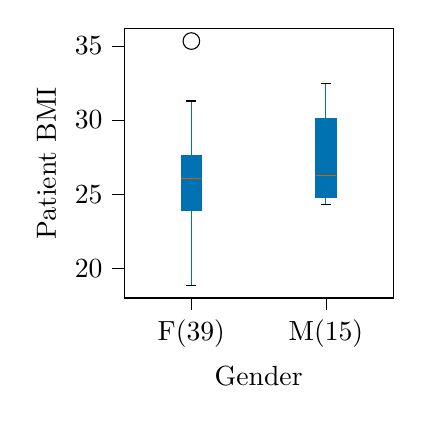
\begin{tikzpicture}

\definecolor{color0}{rgb}{0,0.447058823529412,0.698039215686274}
\definecolor{color1}{rgb}{0.835294117647059,0.368627450980392,0}

\begin{axis}[
height=5cm,
tick align=outside,
tick pos=left,
width=5cm,
x grid style={white!69.0196078431373!black},
xlabel={Gender},
xmin=0.5, xmax=2.5,
xtick style={color=black},
xtick={1,2},
xticklabels={F(39),M(15)},
y grid style={white!69.0196078431373!black},
ylabel={Patient BMI},
ymin=18.0024047239566, ymax=36.1459436746559,
ytick style={color=black}
]
\addplot [color0, opacity=1]
table {%
1 23.8751147842057
1 18.8271110398975
};
\addplot [color0, opacity=1]
table {%
1 27.624520195661
1 31.2809218296147
};
\addplot [black, opacity=1]
table {%
0.9625 18.8271110398975
1.0375 18.8271110398975
};
\addplot [black, opacity=1]
table {%
0.9625 31.2809218296147
1.0375 31.2809218296147
};
\addplot [black, mark=o, mark size=3, mark options={solid,fill opacity=0}, only marks]
table {%
1 35.3212373587151
};
\addplot [color0, opacity=1]
table {%
2 24.7900784908742
2 24.3024870597147
};
\addplot [color0, opacity=1]
table {%
2 30.1080510764016
2 32.4584126587809
};
\addplot [black, opacity=1]
table {%
1.9625 24.3024870597147
2.0375 24.3024870597147
};
\addplot [black, opacity=1]
table {%
1.9625 32.4584126587809
2.0375 32.4584126587809
};
\path [draw=color0, fill=color0]
(axis cs:0.925,23.8751147842057)
--(axis cs:1.075,23.8751147842057)
--(axis cs:1.075,27.624520195661)
--(axis cs:0.925,27.624520195661)
--(axis cs:0.925,23.8751147842057)
--cycle;
\path [draw=color0, fill=color0]
(axis cs:1.925,24.7900784908742)
--(axis cs:2.075,24.7900784908742)
--(axis cs:2.075,30.1080510764016)
--(axis cs:1.925,30.1080510764016)
--(axis cs:1.925,24.7900784908742)
--cycle;
\addplot [color1, opacity=1]
table {%
0.925 26.0261748958953
1.075 26.0261748958953
};
\addplot [color1, opacity=1]
table {%
1.925 26.25
2.075 26.25
};
\end{axis}

\end{tikzpicture}
